Unter dem Oberbegriff des generativen Designs sind verschiedene Methoden zu finden, die sich teilweise stark voneinander unterscheiden. Je nach Branche und Designziel werden unterschiedliche Methoden angewendet. Im Folgenden werden einige aktuelle Designmethoden näher beschrieben.

\label{chap:paramDesign}
\subsection*{Parametrisches Design}
Parametrisches Design ist eine Methode, bei der Modelle auf einer Reihe von Parametern basieren. Diese Parameter sind variabel und können Eigenschaften wie Größe, Form, Proportionen, Materialien und andere designrelevante Merkmale eines Objekts oder einer Struktur repräsentieren. Bei der Anwendung des parametrischen Designs werden zunächst die Parameter festgelegt, die den Raum der möglichen Designs definieren. Anschließend werden Algorithmen oder Regeln entwickelt, die diese Parameter beeinflussen und miteinander in Beziehung setzen. Durch die Manipulation dieser Parameter können Designer verschiedene Variationen und Iterationen des Designs erzeugen. Der große Vorteil des parametrischen Designs liegt in seiner Flexibilität und Effizienz. Indem die Designentscheidungen auf Parameter abgebildet werden, können Änderungen an einem Parameter automatisch zu Änderungen im gesamten Design führen. Dies ermöglicht eine schnelle Exploration verschiedener Designoptionen und eine einfache Anpassung an veränderte Anforderungen.Darüber hinaus ermöglicht das parametrische Design auch die Optimierung von Designs. Durch die Verwendung von Optimierungsalgorithmen können Designer bestimmte Ziele oder Kriterien festlegen, die das Design erfüllen soll. Der Algorithmus sucht dann automatisch nach den besten Parametereinstellungen, um diese Ziele zu erreichen. Parametrisches Design wird vor allem in Branchen eingesetzt, die die Entwicklung komplexer und maßgeschneiderter Designs erfordern und auf spezifische Anforderungen zugeschnitten werden müssen wie in der Architektur oder im Produktdesign.\autocite{2}

\subsection*{Evolutionäre Algorithmen}
Diese Designmethode ist von den Prinzipien der biologischen Evolution inspiriert. Sie ermöglicht die automatisierte Generierung und Optimierung von Designs, indem eine vorher festgelegte Population von Designs erzeugt und iterativ weiterentwickelt wird.
Der Startpunkt ist die erste Population, die aus einer zufälligen Auswahl möglicher Designs basierend auf einem zufälligen Satz von Parametern besteht. Diese Designs werden entweder vom Designer oder von einer KI mit einem \textit{Fitness-Wert} versehen. Alternativ kann der Designer eine eigens programmierte Fitnessfunktion verwenden, in der er die Kriterien und Ziele festlegt, die das Enddesign erfüllen soll. Dadurch wird kein menschlicher Input mehr benötigt, bis ein Ergebnis erzielt wird. Anhand der bewerteten Designs wird dann die zweite Generation von Designs erstellt. Diese zweite Generation erbt die Eigenschaften der Designs aus der ersten Generation, die einen hohen \textit{Fitness-Wert} hatten. Dieser Prozess wird wiederholt, bis ein zufriedenstellendes Ergebnis erreicht ist. Mit jeder Iteration werden die Designs immer besser an die Anforderungen angepasst.\autocite{3}

\subsection*{Generative Adversarial Networks (GANs)}
Bei \ac*{GANs} handelt es sich um zwei konkurrierende Künstliche Neuronale Netzwerke (\ac*{KNN}), die im Austausch miteinander stehen. Ein \ac*{KNN} ist dafür zuständig, reale Designs zu generieren und wird auch als Generator bezeichnet. Das andere \ac*{KNN} ist für die Klassifizierung dieser Designs zuständig und wird als Diskriminator bezeichnet. Der Diskriminator bewertet die generierten Designs nach ihrem Realismus und gibt dieses Feedback an den Generator zurück. Um diese Bewertung durchführen zu können, muss der Diskriminator logischerweise auf realen und generierten Bildern trainiert sein, um den Unterschied zwischen ihnen mit hoher Wahrscheinlichkeit einschätzen zu können. Wie bei den evolutionären Algorithmen verbessern sich die Ergebnisse, die das \ac*{GAN} liefert, mit der Anzahl der Iterationen.\autocite{4}\autocite{11}

\subsection*{Topologieoptimierung}
Bei der Topologieoptimierung handelt es sich um ein Verfahren, bei dem ein Designproblem als ein mathematisches Problem formuliert und von Algorithmen optimiert wird. Das Hauptziel dieses Designverfahrens ist es, solche Designs zu generieren, die den gegebenen Belastungsanforderungen standhalten können und möglichst Gewichtsoptimiert sind. Das wird durch eine Kombination von Künstlicher Intelligenz und Optimierungsalgorithmen realisiert. 

Das Verfahren startet in einem vordefinierten Designraum in dem Parameter für verschiedenste Anforderungen wie Materialeigenschaften, Belastungskriterien und Zielparameter gesetzt werden. Anschließend sucht der Algorithmus nach Bereichen wo Material entfernt werden kann ohne die gesetzten Parameter zu verschlechtern. So entsteht oft organische und filigrane Designs die man in der Topologieoptimierung oft beobachten kann (\autoref{fig:designprozess}). Deshalb wird diese Art von Verfahren insbesondere in Branchen wie der Luft- und Raumfahrt und der Automobilindustrie verwendet, wo diese Eigenschaften von großer Bedeutung sind. \autocite{17}

\begin{figure}[h]
    \centering
    \begin{minipage}{0.5\textwidth}
      \centering
      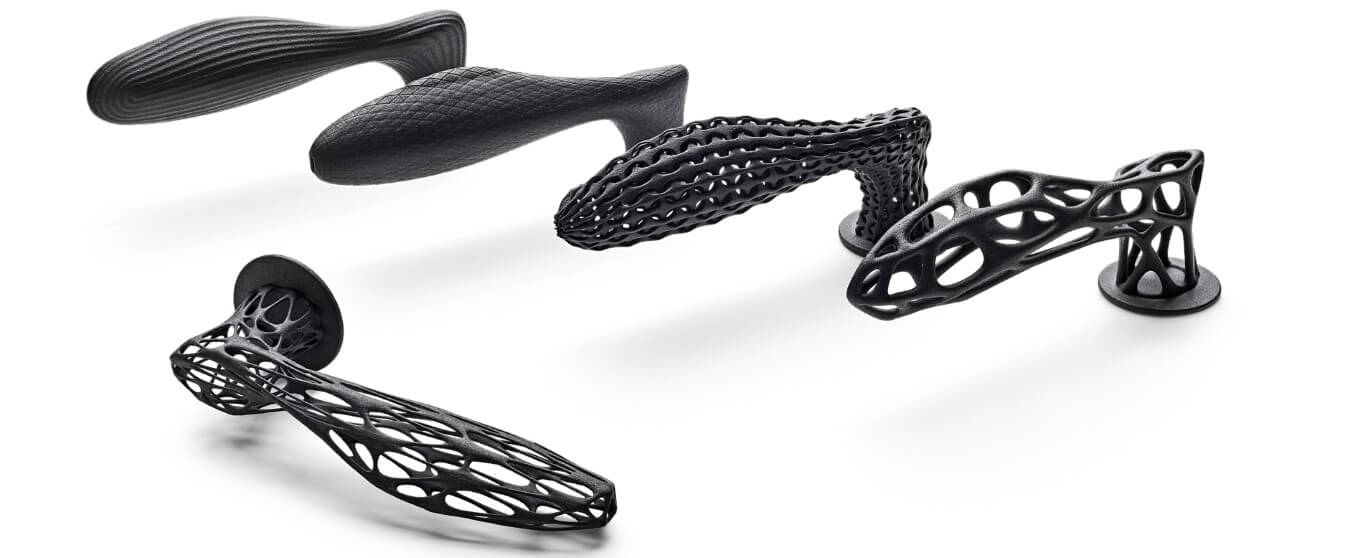
\includegraphics[width=\textwidth]{./images/organicDesign.jpeg}
    \end{minipage}
    \caption{Ein Türgriff mit Topologieoptimierung generiert}
    \label{fig:designprozess}
  \end{figure}